%%%%%%%%%%%%%%%%%%%%%%%%%%%%%%%%%%%%%%%%%%%%%%%%%%%%%%%%%%%%%%%%%%%%%%
% Problem statement
\begin{statement}[
  problempoints=110,
  timelimit=1 sekunda,
  memorylimit=512 MiB,
]{Džumbus}

\setlength\intextsep{-0.1cm}
\begin{wrapfigure}[7]{r}{0.23\textwidth}
\centering
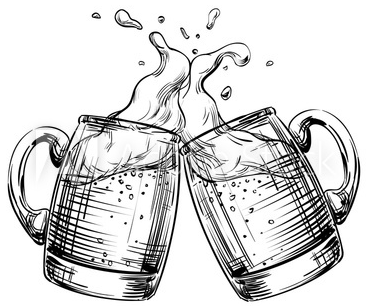
\includegraphics[width=0.23\textwidth]{img/dzumbus.png}
\end{wrapfigure}

Marin je dobar čovjek pa će organizirati čak $Q$ zabava za svojih $N$ prijatelja
-- natjecatelja iz biologije. Na Marinovim će se zabavama posluživati
\textit{džumbus}, mješavina Coca-Cole i soka od đumbira, a zabave se i same
obično pretvore u džumbus.

Marin za svakog prijatelja zna koliko mu je decilitara džumbusa potrebno da se
oraspoloži. Među prijateljima postoji $M$ parova za koje znamo da će se, ako su
na istoj zabavi oba člana para raspoloženi, u nekom trenutku (točnom jednom za
vrijeme te zabave) odvojiti od ostalih i razmijeniti sve bilješke iz biologije
koje posjeduju. Kada osoba $A$ na nekoj zabavi kopira osobi $B$ svoje bilješke
iz biologije, osoba $B$ ih može dijeliti na isti način, no parovi su takvi da
nije moguće da se te bilješke vrate do osobe $A$ \textbf{za vrijeme te zabave,
bez obzira na poredak kojim se parovi sastaju}.

Marin je, u duhu eksperimentiranja, za različite zabave pripremio različite
količine džumbusa. Džumbus će na svakoj zabavi rasporediti među prijateljima
tako da se njih što više na toj zabavi barem jednom upusti u razmjenu bilješki.

Za svaku od $Q$ zabava ispišite koliko će se različitih Marinovih prijatelja na
njoj barem jednom upustiti u razmjenu bilješki.
%%%%%%%%%%%%%%%%%%%%%%%%%%%%%%%%%%%%%%%%%%%%%%%%%%%%%%%%%%%%%%%%%%%%%%
% Input
\subsection*{Ulazni podaci}
U prvom su retku prirodni brojevi $N$ i $M$ iz teksta zadatka. \\
U drugom je retku $N$ prirodnih brojeva $D_i$, količine džumbusa u
decilitrima koje su potrebne Marinovim prijateljima da se oraspolože, redom
od prijatelja s oznakom $1$ do prijatelja s oznakom $N$. \\
U $i$-tom od sljedećih $M$ redaka su po dva prirodna broja $A_i$ i $B_i$
$(A_i \ne B_i)$, oznake parova prijatelja iz teksta zadatka. \\
U sljedećem je retku prirodan broj $Q$ iz teksta zadatka. \\
U sljedećih $Q$ redaka je po jedan prirodan broj $S_i$, količina džumbusa u
decilitrima koju je Marin pripremio za $i$-tu zabavu.


%%%%%%%%%%%%%%%%%%%%%%%%%%%%%%%%%%%%%%%%%%%%%%%%%%%%%%%%%%%%%%%%%%%%%%
% Output
\subsection*{Izlazni podaci}
Ispišite odgovore na $Q$ upita, svaki u svom retku.

%%%%%%%%%%%%%%%%%%%%%%%%%%%%%%%%%%%%%%%%%%%%%%%%%%%%%%%%%%%%%%%%%%%%%%
% Scoring

\subsection*{Bodovanje}
U svim podzadacima vrijedi $1 \le N \le 500$, $1 \le Q \le 2\cdot10^5$ i $1 \le D_i \le 10^9$.

{\renewcommand{\arraystretch}{1.4}
  \setlength{\tabcolsep}{6pt}
  \begin{tabular}{ccl}
 Podzadatak & Broj bodova & Ograničenja \\ \midrule
  1 & 20 & \makecell[l]{$M = N - 1$, $1 \le S_i \le 1000$, \\
            svaki će Marinov prijatelj biti voljan sa najviše dvoje drugih
            prijatelja \\ razmjenjivati bilješke.} \\
  2 & 30 & \makecell[l]{$M = N - 1$, $1 \le S_i \le 10^9$ \\
            svaki će Marinov prijatelj biti voljan sa najviše dvoje drugih
            prijatelja \\ razmjenjivati bilješke.} \\
  3 & 30 & $0 \le M < N$, $1 \le S_i \le 100$ \\
  4 & 30 & $0 \le M < N$, $1 \le S_i \le 10^9$ \\
\end{tabular}}

%%%%%%%%%%%%%%%%%%%%%%%%%%%%%%%%%%%%%%%%%%%%%%%%%%%%%%%%%%%%%%%%%%%%%%
% Examples
\subsection*{Probni primjeri}
\begin{tabularx}{\textwidth}{X'X'X}
\sampleinputs{test/dzumbus.dummy.in.1}{test/dzumbus.dummy.out.1} &
\sampleinputs{test/dzumbus.dummy.in.2}{test/dzumbus.dummy.out.2} &
\sampleinputs{test/dzumbus.dummy.in.3}{test/dzumbus.dummy.out.3}
\end{tabularx}

\textbf{Pojašnjenje trećeg probnog primjera:}
Marin je na prvoj zabavi oraspoložio prijatelje s oznakama
$1$, $2$, $3$, $7$, $9$, $10$, $12$ i $13$ potrošivši na njih
ukupno $45$ decilitara džumbusa.

\setlength\intextsep{-0.5cm}
\begin{wrapfigure}{c}{\textwidth}
\centering
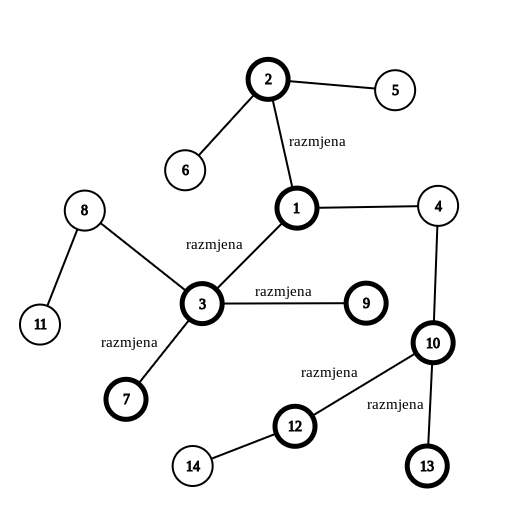
\includegraphics[width=0.6\textwidth]{img/tree.png}
\end{wrapfigure}

%%%%%%%%%%%%%%%%%%%%%%%%%%%%%%%%%%%%%%%%%%%%%%%%%%%%%%%%%%%%%%%%%%%%%%
% We're done
\end{statement}

%%% Local Variables:
%%% mode: latex
%%% mode: flyspell
%%% ispell-local-dictionary: "croatian"
%%% TeX-master: "../hio.tex"
%%% End:
